\chapter{Introduction}
\section{Git}
% VERSION CONTROL SYSTEM
A Version Control System (VSC) is a tool that records changes on your
files over time. The main idea is to keep track of the changes on your
files and to retrieve them later. There are mainly three kinds of 
version control system: local, centralized and distributed. On
a local VCS it is not possible to collaborate with other users and
the structure that keeps track of the files is kept only locally. The
need for collaborations with other users brought the centralized VCS.
On the centralized version control systems there exists a server that keeps
track of the changes on the files and each user pushes and checks out files
from this server. This approach has mainly two problems. The
first is to have a single point of failure, if a server goes down
during a certain time, nobody can check out or pull updates. The
second problem is when you are not connected to the network, you
cannot pull or commit your changes. To solve this problems, the
distributed VCS appeared. Here each user keeps a mirror of the
repository and there is not a central server. An user can always commit
and when connected can push/checkout the changes.\\

%GIT
\emph{Git} \cite{progit}, \cite{gitComm} is a distributed VCS. It was created in 2005 by Linus Torvalds,
for the Linux kernel development. The main difference when comparing to
others distributed VCS is that \emph{git} keeps snapshots of how your system
looks like on a certain moment in time instead of keeping track of
changes.

\section{Motivation}
%OUR PROJECT
Nowadays \emph{git} is having great success. It is efficient, fast and
% in the begin -> when starting unsing it
at first glance, it looks easy to understand and to use. However, When
the users start diving into git, they are sometimes faced with unexpected behavior that
cannot be explained very well. There is not any formal
specification of the operations, like for example, what are the pre-conditions and
what is the result of performing an operation. Normally, when the users
are fronted with a behavior they do not understand, they just learn how to avoid it.\\

%ALLOY
Alloy \cite{Jackson:2006:SAL:1146359} is a formal modeling language, used for describing structures in 
a formal way. After modeling the structures, it is possible to
check for some properties, look for counter examples and to visualize 
instances of the model. \\

The purpose of this project is to
formally model the \emph{git} core using Alloy, analyze it, model some \emph{git}
operations and then check which properties the model does (not)
guarantees. This manual presents to the reader semi-formal description of
\emph{git} internals, the description of some operations and it ends with
some properties that the model guarantees.

The difference between this manual and others \cite{gitComm},\cite{progit}, is
that, before writing it, we tried to understand and model 
the \emph{git} concepts from a formal perspective using Alloy. As result 
we think that our understanding on some key parts of \emph{git}, is more precise
and rigorous. In this manual we try to convey some of that knowledge.

\section{Manual Structure}
%report organization
This reports starts by explaining the organization of \emph{git}, how
it is structured and then we cover each component of \emph{git}:
working directory, index and repository. For matters
of time/space and complexity we focus the object model in the index and in the
repository. After the presentation of the structure we give the semi-formal
specification of some operations. We finish the report with the
analysis of some properties. \\

For a more intuitive explanation, diagrams will be used following
the convention specified in figure \ref{fig:notation}. 

\begin{figure}[tp]
   \centering
   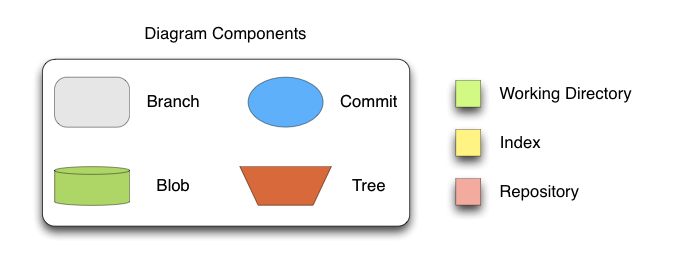
\includegraphics[width=0.8\textwidth]{images/Legenda.png}
   \caption{Convention used in this manual}
   \label{fig:notation}
\end{figure}

